\documentclass[a4paper]{article}
\usepackage[T1]{fontenc}
\usepackage[utf8]{inputenc}
\usepackage[english]{babel}
\usepackage[hidelinks]{hyperref}
\usepackage{graphicx}
\usepackage{times}
\usepackage{amssymb}
\usepackage{amsmath}
\usepackage{wasysym}
\usepackage{pgfplots}
\pgfplotsset{compat=1.3}
\usepackage{fancyvrb}
\usepackage{enumerate}
\fvset{tabsize=3}
\fvset{fontsize=\small}
\newcommand{\code}{\texttt}

\title{\huge{Performance measurements of a small-space Chromatic Polynomial algorithm}}

\author{Mats Rydberg}
\date{\today}

\begin{document}

\maketitle

\begin{abstract}
 The \emph{Chromatic Polynomial} $\chi_G$ of a graph $G$ on $n$ vertices is a univariate polynomial of degree $n$, passing through the points $(k, P_G(k))$ where $P_G(k)$ is the number of $k$-colourings of $G$. In this paper, we present an implementation of the BHKK algorithm which computes $\chi_G$ in time $O^*(2^n)$ and space $O^*(1.2916^n)$. We compare the performance of two different core libraries to eachother and show our performance against the implementation of Haggard et al \cite{haggard} from 2010. We also reproduce the recent results of Beck et al \cite{signed_petersen}, providing the chromatic polynomials of the signed Petersen graphs.
\end{abstract}

\newpage

\section{Introduction}

Presentation

Theory, results, earlier algorithms, history

Intention of this report


The \emph{Chromatic Polynomial} $\chi_G(t)$ of a graph $G$ is a graph invariant describing the colourability of $G$. In particular, the \emph{chromatic number} is the smallest $k$ for which $\chi_G(k) > 0$. It is of high interest in the field of algebraic graph theory, as one of the main artifacts characterizing a graph.

The chromatic polynomial was first in 1912 by Birkhoff, who defined it for planar graphs with the intent on proving the Four Colour Theorem. Whitney extended its definition to general graphs in 1932


Beck et al \cite{signed_petersen} recently presented the chromatic polynomials of the \emph{signed Petersen graphs}. They 

\section{The algorithm}
The algorithm measured in this performance test is described in Björklund et al \cite{cov_pack}, and henceforth referred to as the \textbf{BHKK} algorithm. It is based on the linear-space Fast Zeta Transform described in the same paper, and is proven to perform in time $O(2^n)$ and space $O(1.2916^n)$. 

% The measured theoretical unit of time is the time it takes to perform an addition or a multiplication of two polynomials of degree $n$. The measured theoretical unit of 

Our input is an undirected graph $G$ on $n$ vertices with $m$ edges\footnotemark. The main subroutine counts the number of ways to colour $G$ using $q$ colours. This is done for $q = 0, 1, \ldots n$, yielding $n + 1$ points $(x_i, y_i)$. These are by definition points which the \emph{Chromatic Polynomial} $\chi_G(t)$ passes through. $\chi_G(t)$ has exactly degree $n$, and so we have enough information to recover it explicitly using interpolation.

\footnotetext{Multiple edges and self-edges are two graph invariants that often need special treatment in graph-based algorithms. This is not the case for graph colouring. Any self-edge means the graph is not colourable (a vertex would need to have a different colour from itself), so these are naturally not allowed. In my implementation, I assume they do not exist. Any multiple edge doesn't affect the problem at all, as we are merely considering the \emph{existence} of an edge between two vertices; if there are more than one that doesn't matter.}

The algorithm in pseudo-code as follows:

\begin{enumerate}[{Step} A.]
 \item \label{q} For $q = 0, 1, \ldots, n$, do
 \begin{enumerate}[1.]
  \item Partition $V$ into $V_1$ and $V_2$ of sizes $n_1$ and $n_2$.
  \item \label{step1} For each $X_1 \subseteq V_1$, do
  \begin{enumerate}[a)]
   \item \label{indep1} For each independent $Y_1 \subseteq X_1$, do
$$ h[V_2 \setminus N(Y_1)] \leftarrow h[V_2 \setminus N(Y_1)] + z^{|Y_1|} $$
   \item \label{indep2} For each independent $Y_2 \subseteq V_2$, do
$$ l[Y_2] \leftarrow z^{|Y_2|} $$
   \item $h \leftarrow (h\zeta')\cdot l$
   \item $h \leftarrow h\zeta$
   \item \label{rstep}For each $X_2 \subseteq V_2$, do
$$ r \leftarrow r + (-1)^{n - |X_1| - |X_2|}\cdot h[X_2]^q $$
  \end{enumerate}
  \item Return coefficient $c_n$ of $z^n$ in $r$.
 \end{enumerate}
 \item Construct interpolating polynomial $\chi_G(t)$ on points $(q, c_{nq})$.
 \item Return $\chi_G(t)$.
\end{enumerate}

$N(Y)$ is the set of all vertices in $G$ adjacent to at least one vertex in $Y$, $x\zeta'$ denotes the fast up-zeta transform and $x\zeta$ the fast down-zeta transform (of $x$) (see \cite[sec 2]{cov_pack}. $h$ and $l$ are arrays of size $2^{n_2}$ of polynomials (initialized to zeroes), $r$ is a polynomial. For a more detailed description, see \cite[p 9]{cov_pack}.

\subsection{Optimizations}\label{opts}
Here are presented some improvements to the algorithm that are either natural, mentioned in \cite{cov_pack} or invented by the author. This list is by no means exhaustive, nor is every item critical, but the ones we've explored were proved to be efficient.

\paragraph{Exploiting $q$}
First, we can consider optimizing on the basis of the value of $q$.
\begin{itemize}
\item For $q = 0$, any graph with $n > 0$ can be coloured in 0 ways. For $n = 0$, 0-colouring is undefined. This is a purely semantic question anyway, and empty graphs are not a relevant topic for this paper. This takes $O(1)$ time.
\item For $q = 1$, there are 0 colourings if and only if $|E| > 0$, otherwise there is exactly 1 colouring. This takes $O(n^2)$ time to check, but in practice it is even faster, as we will encounter an edge with high probability before we've scanned the whole graph.
\item For $q = 2$, it is well-known that the graph can be coloured (or found to be non-colourable) in polynomial time using standard techniques (such as breadth-first search).
\end{itemize}

These optimizations will reduce the iterations of the loop at step \ref{q} by three.

\paragraph{$w_{min}(G)$}
A more sophisticated type of optimization involves exploiting the clique number $\omega(G)$, which is a lower bound of the chromatic number $\chi(G)$. Knowing that $\omega(G) \geq a$ for some constant $a$ would allow us to immediately skip all steps~\ref{q} where $q < a$. If $a = n$, we have the complete graph $K_n$, for which $\chi_G$ is known.

Here we define the \emph{density} of a graph $G$ as $dE = m/m_{max} = \frac{2m}{n(n-1)}$. This immediately tells us the \emph{smallest possible} $\omega(G)$. Let us call it $\omega_{min}(G)$. In fact, the following holds:

\begin{equation}\label{omega}
\omega_{min}(G) = \left\{ \begin{array}{lll}
                           n - a & \text{if } m = m_{max} - a & 0 \leq a < \lfloor\frac{n}{2}\rfloor \\
                           \lceil\frac{n}{2}\rceil - a & \text{if } \lfloor(\frac{n}{2})^2\rfloor < m \leq m_{max} - (a + 1)\lfloor\frac{n}{2}\rfloor & 0 \leq a \leq \lfloor\frac{n}{2}\rfloor - 2 \\
                           2 & \text{if } 0 < m \leq \lfloor(\frac{n}{2})^2\rfloor & \\
                           1 & \text{if } m = 0 & \\
                          \end{array}
                  \right.
\end{equation}

As we can see from the equation, only graphs with $m > \lfloor(\frac{n}{2})^2\rfloor$ provides $\omega_{min}(G) > 2$ and for $q \leq 2$ we already have good optimizations. So how dense is a graph where this bound on $m$ holds? Let us specify the threshold density $T_{dE}(n)$ as

$$
T_{dE}(n) = \frac{\lfloor(\frac{n}{2})^2\rfloor}{m_{max}} = 2\frac{\lfloor(\frac{n}{2})^2\rfloor}{n(n-1)} = \left\{ \begin{array}{ll}
          \frac{n}{2(n-1)} & \text{if } n \text{ even}\\
          \frac{n + 1}{2n} = T_{dE}(n+1) & \text{if } n \text{ odd}\\
          \end{array}
  \right.
$$

In conclusion, any graph with $dE > T_{dE}(n)$ can optimize away at least one additional computation of step~\ref{q} above. It also follows that as $n \rightarrow \infty$ we will have $T_{dE}(n) \rightarrow \frac{1}{2}$. The following plot shows how fast we converge for the graphs discussed in this paper.

\begin{center}
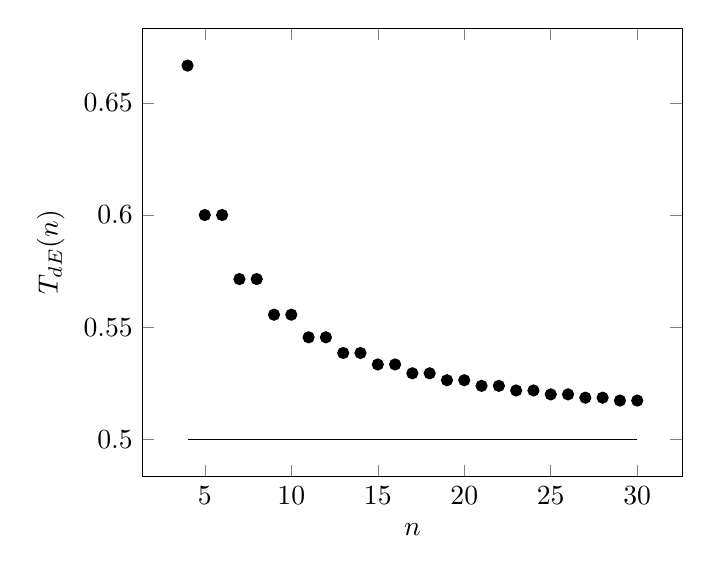
\begin{tikzpicture}
\begin{axis}[%samples at={4,5,6,7,8,9,10,11,12,13,14,...,23},
xlabel=$n$,
ylabel=$T_{dE}(n)$]
%\addplot[black, mark=*, samples=20, domain=4:23] {(2*floor((x/2)^2))/(x*(x-1))};
\addplot[black, only marks, mark=*, samples=14, domain=4:30] {x/(2*(x-1))};
\addplot[black, only marks, mark=*, samples=13, domain=5:29] {(x+1)/(2*x)};
\addplot[black, samples=10, domain=4:30] {1/2};
\end{axis}
\end{tikzpicture}
\end{center}

This result is quite interesting, because for larger graphs, we have a smaller $T_{dE}(n)$, which gives us a higher probability to be able to optimize, and it is also for larger graphs that we are most interested in optimizing techniques. For a graph with $n=23$ and $dE = 75$, we would be able to skip evaluating $q\leq7$, which would yield an expected decrease in time by about 15\%\footnotemark. %TODO update this number 
%UPDATED 1/11 from two tests on pari-0.2 and pari-0.2.1 and graphs 17_80 and 19_85.

\footnotetext{This number is based on experimental results presented below.}

\paragraph{Parallelization} Most importantly, and also mentioned in \cite{cov_pack}, is to parallelize computations of step \ref{step1}, as these are independent of eachother. This would yield significant time improvements in theory. With access to $2^{|V_1|}$ processors, we would be able to execute the program in time $O(1.5486^n)$. Typically, we will only have access to a constant number of processors in practice, allowing each of them to execute a range of iterations of step \ref{step1}. As presented below, we can expect to reduce the time consumption of the program by a factor of around 6. %TODO: make sure this number is correct.

We may also parallelize the steps \ref{q} on $O(n)$ parallel CPUs. This would not reduce the exponential factor of the time complexity, but it does reduce the polynomial factor and it is likely to give significant results in practice. I do not investigate this optimization technique, as my resources are already exhausted by parallelizing step \ref{step1}.

\paragraph{Caching} Since in fact all steps of the inner loop of BHKK are independent from $q$, except the final step~\ref{rstep}, we are actually re-computing the same values for the array $h$ as we increase $q$. If we would cache these values after the first call of step~\ref{step1}, we would be performing only step~\ref{rstep} for all the rest of the computations, plus a look-up in our cache table. This would require a cache of size $2^{n_1} 2^{n_2} = 2^n$.



\section{Implementation details}
My implementation only partially supports $n > 64$. In practice, the program does not perform very well for such large problems anyway, so this restriction is not critical. This allows me to use a natural way of encoding a set by simply letting it be a whole integer word, 64 bits long. A one in position $i$ of the word means that vertex $i$ of $G$ is present in the set represented by the word.

% I've chosen to support adjacency matrices as input structure, representing an arbitrary graph. Another common graph representation is the edge list, which is faster, but since our problem is exponentially hard, another degree of a polynomial term doesn't really affect our performance very much. It is also more straight-forward for me to generate randomized graphs using an adjacency matrix.

For polynomial representation I've emplyed the use of two libraries for number theoretic calculations. These also provide interpolation functionality.

\subsection{NTL 6.0.0}
The first is NTL, Number Theoretic Library, written in C++ by Victor Shoup at New York University\cite{ntl}. It is advertised as one of the fastest implementations of polynomial arithmetics, which is all that I am interested in. Unfortunately, it does not provide any non-trivial way of exponentiating polynomials, and its multiplication algorithms are a bit lackluster after some careful studying. It is very easy to use, provides its own garbage collection and has a rich, high-level interface for library usage.

The functions I use are primarily these: 

\begin{itemize}
 \item \code{ZZX.operator+=()}
 \subitem Addition and assignment for polynomials. %TODO Documentation citation
 \item \code{ZZX.operator*=()}
 \subitem Multiplication and assignment for polynomials. %TODO Doc citation
\end{itemize}

Binaries are called \code{bhkk-ntl-x.y.z}.

\subsection{PARI 2.5.5}
Experiencing the relative lack of performance boost from the NTL implementation led me to find also the PARI project. It is written in C mainly by a group of French computer scientists at Université Bordeaux \cite{pari}, together with a calculator-like interface (\code{gp}) to be used by an end-user (comparable to Maple). The PARI library is provided at a much lower level, requires the user to garbage collect (since it is written in C, after all), has a much steeper learning curve and a very detailed but hard-to-grasp documentation. PARI provides special methods for exponentiation of polynomials, but it is a bit unclear how these are implemented exactly.

The functions I use are primarily these: 

\begin{itemize}
 \item \code{ZX\_add()}
 \subitem Addition for polynomials. %TODO: doc citation
 \item \code{ZX\_mul()}
 \subitem Multiplication for polynomials. %TODO: citation from documentation
 \item \code{gpowgs()}
 \subitem General exponentiation for PARI types. Used for polynomials.
\end{itemize}

Binaries are called \code{bhkk-pari-x.y.z}.


%TODO: is this part necessary?
%The PARI library implements its own stack, which it needs to have allocated before any function calls can be made. Preferably, a large enough stack should be allocated at the start of the program, so that re-allocations will not be necessary. I am allocating 50MB of memory for the stack, which is more than enough for most instances. This has a side effect in the measurements of memory usage, meaning that the virtual memory peak is constant for all PARI executions.

\subsection{GMP 5.1.2}
Both the libraries I use to represent polynomials allow (and encourage) the user to configure them using GMP\cite{gmp} as the low-level interface for integral arithmetic (actually, for all arithmetic, but I only use integers). Authors of both libraries suggest that using GMP instead of their own, native low-level interface will yield significant performance boosts. For this reason, I have done just that. GMP is well documented, easy-to-use, provides both C and C++ interfaces and even has a well-maintained bug reporting facility (I got an answer the same day!). GMP allows the user a rich variety of configuration options, and I've tried to optimize as narrowly as possible to get maximum performance on one machine.

In my implementation, I only use GMP to generate randomized graphs. All arithmetic is performed via the interfaces of PARI and NTL, which themselves call underlying GMP functions.

\section{Algorithm performance parameters}
The algorithm has some perks that make it perform better or worse for different input. In this section I aim to explore a few of these characteristics.

\subsection{Sparse and dense graphs}\label{sparsedense}
The algorithm in itself is designed in a way that allow for a smaller degree of complexity for \emph{dense} graphs. This is in contrast to many of the algorithms which I've studied for graph colouring problems. And this is not only for very dense graphs, but performance is in fact a function that is directly related to graph density, and consistently performs better for every additional edge to a graph. This follows directly from steps \ref{indep1} and \ref{indep2} above:

$$ h[V_2 \setminus N(Y_1)] \leftarrow h[V_2 \setminus N(Y_1)] + z^{|Y_1|} $$

$$ l[Y_2] \leftarrow z^{|Y_2|} $$

Recall that these lines will only be executed for \emph{independent} sets $Y_1$ and $Y_2$. As graph density increases, fewer subsets of the vertex set $V$ will be independent, and fewer of these lines will be executed. This has a direct effect in reducing some additions and assignments, but more importantly has side effects in all subsequent steps. 
%Addition-assignment with zero is a non-operation. Multiplication with zero is trivial, and yields even more zeroes. In the extreme case of a complete graph $G=(V,E)$, where all independent subsets of $V$ are of size 1, the most time-critical operation may be the independence testing function (which is executed on all subsets regardless of $G$).

% This discussion of course also applies to \emph{sparse} graphs, in which case we will have \emph{fewer} zeroes and more non-trivial operations.

\subsection{Multiplication algorithms}
%TODO: Count number of multiplications/additions/powerings
Much of the complexity of the whole algorithm comes down to how polynomial multiplication is performed. The most common operation is to multiply two polynomials of \emph{small} degree but with \emph{large} coefficients. This is because the degree of the polynomials increase as $O(n)$ while their coefficients increase as $O(2^n)$. %TODO: Citation?

% Trivially, a polynomial multiplication would be to expand over both operands' coefficients and cross-multiply them in a standard fashion. This is very inefficient, and many techniques have been developed to deal with this problem. In fact, the original issue has always been to multiply two large integers, but the most sophisticated results show methods that make use of polynomials for this purpose. The algorithm with the best asymptotic complexity is the Schönhage-Strassen algorithm \cite{strass}, but it has a large overhead and becomes useful only for huge operands. It is based on a Fast Fourier Transform. The most go-to algorithm is the Toom-Cook \cite{toom-cook} (aka Toom-$k$) family, in which Toom-2 (aka Karatsuba) or Toom-3 are the most common.

% The technique used in Toom-$k$ for multiplying two large integers is to split them up in parts, introduce a polynomial representation of degree $k-1$ for these parts (the parts are coefficients), evaluate the polynomials at certain points (the choice of points is critical%TODO: citation!
% ), perform pointwise multiplication of the evaluated polynomials, interpolate the resulting points into a resulting polynomial, and finally reconstruct the integer from the coefficients of the resulting polynomial. This technique is easily translated for polynomial multiplication as well, where the first and last steps would be skipped.

The GMP library supports Karatsuba, Toom-3, Toom-4, Toom-6.5, Toom-8.5 and Schönhage-Strassen \cite[p 90]{gmp}, which means all libraries used in my programs uses these algorithms \emph{at least} when multiplying integers (ie, coefficients of polynomials).

NTL implements Karatsuba, Schönhage-Strassen and another FFT-based technique for polynomials \cite{ntl_zzx}.

I have not found any documentation specifying which algorithms are implemented in the PARI library for polynomial multiplication. From analyzing the source code, it seems as if PARI ''converts'' the polynomial to an integer and submits it to its integer multiplication function (which would be one of GMPs).

\section{Experimental results}
This section presents selected results in three parts. First, we show the metrics for the best implementation currently available, and discuss how it relates to the theory described above. Second, we compare it to some of the other implementations, to visualize the impact of each development choice. Most importantly, we make a comparison between which library for polynomial arithmetic was used. Thirdly, we compare our results to the Haggard-Pearce-Royle implementation \cite{haggard} and reproduce the results of Beck et al\cite{signed_petersen}. We end by providing the chromatic polynomial for a famous graph.

For the first two parts, the tests are performed on randomized graphs, generated for some values of $n$ and $dE$ using a tool developed by the author. The process is basically to fill an array $A$ of size $m_{max} = \frac{n(n-1)}{2}$ with $m$ ones and rest zeroes, shuffle $A$ using Fisher-Yates shuffle and then add the edge $v_iv{i+1}$ to the graph if $A[i] = 1$.

\subsection{Measurements}
All tests are performed on the same machine, with the following specifications.

\begin{center}
\begin{tabular}{l|l}
CPU (cores, threads) & Intel i7-3930K 3.2GHz (6, 12) \\ 
OS & GNU/Linux 3.8.13.4-desktop-1.mga3 (Mageia 3) x86\_64 \\ 
Memory & 16GB DDR3 1333Mhz \\ 
Compilator & GCC 4.7.2 (g++) \\ 
\end{tabular}
\end{center}

For all time and memory measurements, the GNU time 1.7 program is used \cite{time}. The user time, elapsed time (real time)\footnotemark and peak resident set size are the data points recovered as measurements. These measurements are taken by running the specified program on 100 graphs of equal size and the average values are the ones presented.

\footnotetext{Do note that for single-threaded applications, user time and real time are (more or less) the same. No graphs are therefore provided for the real time measurements. The ''less'' refers to the fact that there are some units of time scheduled as system time, but these values are too small to be significant in these experiments.}

\subsection{\code{bhkk-pari-0.3}}
The most powerful implementation is called \code{bhkk-pari-0.3}. It implements these optimizations: $q = 0, 1$, $w_{min}(G)$, parallelization. We show here its time and memory consumption in relation to both $n$ and $dE$.

\begin{center}
\begin{tabular}{rl}
\begin{tikzpicture}
\begin{axis}[title={Random graphs of fized density},
legend pos=north west,baseline,trim axis left,small,
xlabel=$n$,
ylabel=Average real time (ms)]
\addplot[red,mark=triangle*] table[x=n,y=rt] {tables/bhkk-pari-0.3_1};
\addplot[blue,mark=asterisk] table[x=n,y=rt] {tables/bhkk-pari-0.3_2};
\addplot[black, domain=4:23] {(1/100)*x*2^x};
\legend{$dE = 40$, $dE = 75$, $f_t$}
\end{axis}
\end{tikzpicture}
&
\begin{tikzpicture}
\begin{axis}[title={Random graphs of fized density},
legend pos=north west,baseline,trim axis right,small,
yticklabel pos=right, ylabel style={align=right},
xlabel=$n$,
ylabel=Average peak resident set size (kB)]
\addplot[red,mark=triangle*] table[x=n,y=rss] {tables/bhkk-pari-0.3_1};
\addplot[blue,mark=asterisk] table[x=n,y=rss] {tables/bhkk-pari-0.3_2};
\addplot[black, domain=4:23] {(32)*(1.2916)^x + 10000};
\legend{$dE = 40$, $dE = 75$, $f_m$}
\end{axis}
\end{tikzpicture}
\\
\begin{tikzpicture}
\begin{axis}[title={Random graphs of fixed $n$},
legend pos=north west,baseline,trim axis left,small,
xlabel=$dE$,
ylabel=Average real time (ms)]
\addplot[red,mark=triangle*] table[x=dE,y=rt] {tables/bhkk-pari-0.3_3};
% \addplot[black, domain=4:23] {(1/100)*x*2^x};
% \legend{lol, $f_t$}
\end{axis}
\end{tikzpicture}
&
\begin{tikzpicture}
\begin{axis}[title={Random graphs of fixed $n$},
legend pos=north west,baseline,trim axis right,small,
yticklabel pos=right, ylabel style={align=right},
xlabel=$dE$,
ylabel=Average peak resident set size (kB)]
\addplot[red,mark=triangle*] table[x=dE,y=rss] {tables/bhkk-pari-0.3_3};
% \addplot[black, domain=4:23] {(32)*(1.2916)^x + 10000};
% \legend{lol, $f_m$}
\end{axis}
\end{tikzpicture}
\\
\end{tabular}
\end{center}

%TODO: Some comments on the results.

\subsection{Practical improvements}
Here ''dense'' means $dE = 75$ and ''sparse'' means $dE = 40$.

First we show the performance improvements for the three specifications implementations linked to the PARI library, versions 0.1, 0.2 and 0.3. 0.2 implemented parallelization.

\begin{center}
\begin{tabular}{rl}
\begin{tikzpicture}
\begin{axis}[title={Random dense graphs},
legend pos=north west,baseline,trim axis left,small,
xlabel=$n$,
ylabel=Average real time (ms)]
\addplot[blue,mark=asterisk] table[x=n,y=rt] {tables/bhkk-pari-0.1_2};
\addplot[blue,mark=asterisk] table[x=n,y=rt] {tables/bhkk-pari-0.2_2};
\addplot[red,mark=triangle*] table[x=n,y=rt] {tables/bhkk-pari-0.3_1};
% \addplot[black, domain=4:23] {(1/100)*x*2^x};
\legend{0.1, 0.2, 0.3}
\end{axis}
\end{tikzpicture}
&
\begin{tikzpicture}
\begin{axis}[title={Random dense graphs},
legend pos=north west,baseline,trim axis right,small,
yticklabel pos=right, ylabel style={align=right},
xlabel=$n$,
ylabel=Average peak resident set size (kB)]
\addplot[blue,mark=asterisk] table[x=n,y=rss] {tables/bhkk-pari-0.1_2};
\addplot[blue,mark=asterisk] table[x=n,y=rss] {tables/bhkk-pari-0.2_2};
\addplot[red,mark=triangle*] table[x=n,y=rss] {tables/bhkk-pari-0.3_1};
% \addplot[black, domain=4:23] {(32)*(1.2916)^x + 10000};
\legend{0.1, 0.2, 0.3}
\end{axis}
\end{tikzpicture}
\\
\begin{tikzpicture}
\begin{axis}[title={Random sparse graphs},
legend pos=north west,baseline,trim axis left,small,
xlabel=$n$,
ylabel=Average real time (ms)]
\addplot[blue,mark=asterisk] table[x=n,y=rt] {tables/bhkk-pari-0.1_1};
\addplot[blue,mark=asterisk] table[x=n,y=rt] {tables/bhkk-pari-0.2_1};
\addplot[red,mark=triangle*] table[x=n,y=rt] {tables/bhkk-pari-0.3_2};
% \addplot[black, domain=4:23] {(1/100)*x*2^x};
\legend{0.1, 0.2, 0.3}
\end{axis}
\end{tikzpicture}
&
\begin{tikzpicture}
\begin{axis}[title={Random sparse graphs},
legend pos=north west,baseline,trim axis right,small,
yticklabel pos=right, ylabel style={align=right},
xlabel=$n$,
ylabel=Average peak resident set size (kB)]
\addplot[blue,mark=asterisk] table[x=n,y=rss] {tables/bhkk-pari-0.1_1};
\addplot[blue,mark=asterisk] table[x=n,y=rss] {tables/bhkk-pari-0.2_1};
\addplot[red,mark=triangle*] table[x=n,y=rss] {tables/bhkk-pari-0.3_2};
% \addplot[black, domain=4:23] {(32)*(1.2916)^x + 10000};
\legend{0.1, 0.2, 0.3}
\end{axis}
\end{tikzpicture}
\\
\begin{tikzpicture}
\begin{axis}[title={Random graphs, $n = 19$},
legend pos=north west,baseline,trim axis left,small,
xlabel=$dE$,
ylabel=Average real time (ms)]
\addplot[blue,mark=asterisk] table[x=dE,y=rt] {tables/bhkk-pari-0.1_3};
\addplot[blue,mark=asterisk] table[x=dE,y=rt] {tables/bhkk-pari-0.2_5};
\addplot[red,mark=triangle*] table[x=dE,y=rt] {tables/bhkk-pari-0.3_3};
% \addplot[black, domain=4:23] {(1/100)*x*2^x};
\legend{0.1, 0.2, 0.3}
\end{axis}
\end{tikzpicture}
&
\begin{tikzpicture}
\begin{axis}[title={Random graphs, $n = 19$},
legend pos=north west,baseline,trim axis right,small,
yticklabel pos=right, ylabel style={align=right},
xlabel=$dE$,
ylabel=Average peak resident set size (kB)]
\addplot[blue,mark=asterisk] table[x=dE,y=rss] {tables/bhkk-pari-0.1_3};
\addplot[blue,mark=asterisk] table[x=dE,y=rss] {tables/bhkk-pari-0.2_5};
\addplot[red,mark=triangle*] table[x=dE,y=rss] {tables/bhkk-pari-0.3_3};
% \addplot[black, domain=4:23] {(32)*(1.2916)^x + 10000};
\legend{0.1, 0.2, 0.3}
\end{axis}
\end{tikzpicture}
\\
\end{tabular}
\end{center}

All parallelized runs are executed using 45 virtual threads. Of course, the test machine only allows 12 threads in parallel, but experiments have shown that using 45 threads costs less time and more memory. For the sake of brevity, these results are omitted from this paper.

\subsubsection{NTL}
To provide a little insight in how important the actual implementation of polynomial arithmetic is, we also show a comparison of the implementation linked with PARI and the one linked with NTL.

\begin{center}
\begin{tabular}{rl}
\begin{tikzpicture}
\begin{axis}[title={Random dense graphs},
legend pos=north west,baseline,trim axis left,small,
xlabel=$n$,
ylabel=Average real time (ms)]
\addplot[red,mark=triangle*] table[x=n,y=rt] {tables/bhkk-pari-0.3_1};
\addplot[blue,mark=asterisk] table[x=n,y=rt] {tables/bhkk-ntl-0.3_1};
% \addplot[black, domain=4:23] {(1/100)*x*2^x};
\legend{\code{bhkk-pari-0.3}, \code{bhkk-ntl-0.3}, $f_t$}
\end{axis}
\end{tikzpicture}
&
\begin{tikzpicture}
\begin{axis}[title={Random dense graphs},
legend pos=north west,baseline,trim axis right,small,
yticklabel pos=right, ylabel style={align=right},
xlabel=$n$,
ylabel=Average peak resident set size (kB)]
\addplot[red,mark=triangle*] table[x=n,y=rss] {tables/bhkk-pari-0.3_1};
\addplot[blue,mark=asterisk] table[x=n,y=rss] {tables/bhkk-ntl-0.3_1};
% \addplot[black, domain=4:23] {(32)*(1.2916)^x + 10000};
\legend{\code{bhkk-pari-0.3}, \code{bhkk-ntl-0.3}, $f_m$}
\end{axis}
\end{tikzpicture}
\\
\end{tabular}
\end{center}

The results are consistently in significant favour of PARI.

\subsection{Relation to other work}


\subsection{PARI 2.5.5}
% Some text about PARI. %TODO

\subsubsection{Increasing $n$}

This is time as a function of $n$. Expected function in theory is $O^*(2^n)$. For comparison, I also plot the function $f_t(n) = \frac{n}{100} 2^n$, which is a model of the time usage of the algorithm, where each measured operation takes a hundredth of a millisecond, providing the desired asymptotical behaviour.

\begin{center}
\begin{tabular}{rl}
\begin{tikzpicture}
\begin{axis}[title={0.1},
legend pos=north west,baseline,trim axis left,small,
xlabel=$n$,
ylabel=CPU time (ms)]
\addplot[red,mark=triangle*] table[x=n,y=ut] {./tables/bhkk-pari-0.1_1};
\addplot[blue,mark=asterisk] table[x=n,y=ut] {tables/bhkk-pari-0.1_2};
\addplot[black, domain=4:23] {(1/100)*x*2^x};
\legend{Dense, Sparse, $f_t$}
\end{axis}
\end{tikzpicture}
&
\begin{tikzpicture}
\begin{axis}[title={0.2},
legend pos=north west,baseline,trim axis right,small,
yticklabel pos=right, ylabel style={align=right},
xlabel=$n$,
ylabel=CPU time (ms)]
\addplot[red,mark=triangle*] table[x=n,y=ut] {tables/bhkk-pari-0.2_1};
\addplot[blue,mark=asterisk] table[x=n,y=ut] {tables/bhkk-pari-0.2_2};
\addplot[black, domain=4:23] {(1/100)*x*2^x};
\legend{Dense, Sparse, $f_t$}
\end{axis}
\end{tikzpicture}
\\
\begin{tikzpicture}
\begin{axis}[title={0.2},
legend pos=north west,baseline,trim axis left,small,
xlabel=$n$,
ylabel=Real time (ms)]
\addplot[red,mark=triangle*] table[x=n,y=rt] {tables/bhkk-pari-0.2_1};
\addplot[blue,mark=asterisk] table[x=n,y=rt] {tables/bhkk-pari-0.2_2};
\addplot[black, domain=4:23] {(1/100)*x*2^x};
\legend{Dense, Sparse, $f_t$}
\end{axis}
\end{tikzpicture}
&
\begin{tikzpicture}
\begin{axis}[title={0.1 vs 0.2, dense graphs},
legend pos=north west,baseline,trim axis right,small,
yticklabel pos=right, ylabel style={align=right},
xlabel=$n$,
ylabel=Real time (ms)]
\addplot[red,mark=triangle*] table[x=n,y=rt] {tables/bhkk-pari-0.1_1};
\addplot[blue,mark=triangle*] table[x=n,y=rt] {tables/bhkk-pari-0.2_1};
\addplot[black, domain=4:23] {(1/100)*x*2^x};
\legend{\code{aka}, \code{midori}, $f_t$}
\end{axis}
\end{tikzpicture}
\\
\end{tabular}
\end{center}

The results are not revealing much that was not expected. We can see that 0.1 actually uses more CPU time than 0.1 (top graphs), some of which could be contributed to the fact that parallelization requires some overhead. 

Next we have memory usage as a function of $n$. Expected function from theory is $O^*(1.2916^n)$. Our modeling function is $f_m(n) = 32\cdot1.2916^n + 10000$, which assumes an overhead of 10,000kB and each measured element using up 32kB on average. Since a parallelized program uses also memory in parallel, we also employ the modeling function $f_m^{12}(n) = 12\cdot32\cdot1.2916^n + 10000$, assuming 12 threads in parallel using maximum memory.

\begin{center}
\begin{tabular}{rl}
\begin{tikzpicture}
\begin{axis}[title={0.1},
legend pos=north west,trim axis left,small,
xlabel=$n$,
ylabel=Peak resident set size (kB)]
\addplot[red,mark=triangle*] table[x=n,y=rss] {./tables/bhkk-pari-0.1_1};
\addplot[blue,mark=asterisk] table[x=n,y=rss] {tables/bhkk-pari-0.1_2};
\addplot[black, domain=4:23] {(32)*(1.2916)^x + 10000};
\legend{Dense, Sparse, $f_m$}
\end{axis}
\end{tikzpicture}
&
\begin{tikzpicture}
\begin{axis}[title={0.2},
legend pos=north west,trim axis right,small,
yticklabel pos=right, ylabel style={align=right},
xlabel=$n$,
ylabel=Peak resident set size (kB)]
\addplot[red,mark=triangle*] table[x=n,y=rss] {tables/bhkk-pari-0.2_1};
\addplot[blue,mark=asterisk] table[x=n,y=rss] {tables/bhkk-pari-0.2_2};
\addplot[black, domain=4:23] {(12)*(32)*(1.2916)^x + 10000};
\legend{Dense, Sparse, $f_m^{12}$}
\end{axis}
\end{tikzpicture}
\\
\begin{tikzpicture}
\begin{axis}[title={0.1 vs 0.2, dense graphs},
legend pos=north west,trim axis left,small,
xlabel=$n$,
ylabel=Peak resident set size (kB)]
\addplot[red,mark=triangle*] table[x=n,y=rss] {tables/bhkk-pari-0.1_1};
\addplot[blue,mark=triangle*] table[x=n,y=rss] {tables/bhkk-pari-0.2_1};
% \addplot[black, domain=4:23] {(32)*(1.2916)^x + 10000};
\legend{0.1, 0.2}
\end{axis}
\end{tikzpicture}
&
\begin{tikzpicture}
\begin{axis}[title={0.1 vs 0.2, normalized},
legend pos=north west,trim axis right,small,
yticklabel pos=right, ylabel style={align=right},
xlabel=$n$,
ylabel=Peak resident set size (kB)]
\addplot[red,mark=triangle*] table[x=n,y=rss] {tables/bhkk-pari-0.1_1};
\addplot[blue,mark=triangle*] table[x=n,y expr=\thisrow{rss}/12 + (11/12)*10000] {tables/bhkk-pari-0.2_1};
\addplot[black, domain=4:23] {(32)*(1.2916)^x + 10000};
\legend{0.1, 0.2, $f_m$}
\end{axis}
\end{tikzpicture}
\\
\end{tabular}
\end{center}

The ''normalization'' used above follows the model in an attempt to isolate the peak resident set usage by the most memory-expensive thread of 0.2. The measured value $mem$ is divided by $t = 12$ and then we add the number $\frac{t-1}{t}\cdot 10000$ to compensate for our modelled overhead.

\subsubsection{Parallelization}

Here we investigate how our parallelization scheme acts as we increase the number of threads. We plot the function of user and real time as we increase the number of threads. Recall that our maximum \emph{actual} parallelization width is 12.

\begin{center}
\begin{tabular}{rl}
\begin{tikzpicture}
\begin{axis}[title={0.2},
legend pos=south east,trim axis left,small,
xlabel=\# threads,
ylabel=CPU time (ms)]
\addplot[red, mark=|] table[x=t,y=ut] {tables/bhkk-pari-0.2_3};
\addplot[blue, mark=x] table[x=t,y=ut] {tables/bhkk-pari-0.2_4};
\legend{Dense, Sparse}
\end{axis}
\end{tikzpicture}
&
\begin{tikzpicture}
\begin{axis}[title={0.2},
legend pos=north east,trim axis right,small,
yticklabel pos=right, ylabel style={align=right},
xlabel=\# threads,
ylabel=Real time (ms)]
\addplot[red, mark=|] table[x=t,y=rt] {tables/bhkk-pari-0.2_3};
\addplot[blue,mark=x] table[x=t,y=rt] {tables/bhkk-pari-0.2_4};
\legend{Dense, Sparse}
\end{axis}
\end{tikzpicture}
\\
\end{tabular}
\end{center}

There seem to be no notable difference in how sparse and dense graphs parallelize. As expected, the plots peak at 12 threads in the first figure. What is not expected is that the top performance was measured for around 45 threads (this is also the reason why I have more data points between 40 and 50). It is not hard to realize that some threads will terminate much sooner than others (because they happened to get a range of subsets which were more frequently independent, see section \ref{sparsedense}), and so using > 12 threads could be useful. It is unclear why our best results come around 45, however.

%TODO Make another test with different n

Another interesting note to take is that for 100 threads, processing the dense graph take more time than the sparse graph. This can partly be explained by the fact that the OS is now spending lots of time context switching the 100 threads over the 12 CPUs, but from a more algorithmic point of view, we can make another argument. 

As we let each thread iterate over fewer and fewer subsets from step \ref{step1}, our real time consumption is more and more dominated by the one thread that takes the longest time to execute. That is, the thread that was allocated with the ''worst'' range of subsets (the one with the least dependencies). ''Bad'' ranges are more common when the graph is sparse, but as we divide the subsets into smaller ranges, the ''worst'' range decreases in ''badness'' faster for a sparse graph than for a dense. In fact, the probability that a selected range of subsets from a dense graph includes more independent sets to consider than any selected range from a sparse graph is higher for moderate range sizes (it stays $< 0.5$, of course), even though it approaches zero as we approach range size one.

\begin{center}
\begin{tabular}{rl}
\begin{tikzpicture}
\begin{axis}[title={\code{midori}},
legend pos=north west,trim axis left,small,
xlabel=\# threads,
ylabel=Peak resident set size (kB)]
\addplot[red, mark=|] table[x=t,y=rss] {tables/bhkk-pari-0.2_3};
\addplot[blue, mark=x] table[x=t,y=rss] {tables/bhkk-pari-0.2_4};
\legend{Dense, Sparse}
\end{axis}
\end{tikzpicture}
&
\begin{tikzpicture}
\begin{axis}[title={\code{midori}},
legend pos=north east,trim axis right,small,
yticklabel pos=right, ylabel style={align=right},
xlabel=\# threads,
ylabel=Average resident set size per thread (kB)]
\addplot[red, mark=|] table[x=t,y expr=\thisrow{rss} / x] {tables/bhkk-pari-0.2_3};
\addplot[blue,mark=x] table[x=t,y expr=\thisrow{rss} / x] {tables/bhkk-pari-0.2_4};
\legend{Dense, Sparse}
\end{axis}
\end{tikzpicture}
\\
\end{tabular}
\end{center}

The memory usage increases quite linearly as we add threads. This is due to the fact that \code{midori} stores all the $t$ intermediate return values simultaneously until all threads are ready. The average memory per thread seems to converge to some constant.

\bigskip

When we use $t$ threads, in theory we should be able to compute the same problem $t$ times faster than if we use 1 thread. This is not the case in practice, as we have seen so far. But how much do we actually gain? Let's define a parallelization factor $p$ as the quotient between the time used by \code{aka} and the time used by \code{midori}.

\begin{center}
\begin{tikzpicture}
\begin{axis}[title={Dense graphs},
legend pos=south east,trim axis right,small,
xlabel=$n$,
ylabel=$p$]
\addplot[blue,mark=triangle*] table[x=n,y expr = \thisrow{0.1} / \thisrow{0.2}] {tables/bhkk-pari-0.x_rtimes};
\legend{\code{aka} / \code{midori}}
\end{axis}
\end{tikzpicture}
\end{center}

By the measured data, $p$ stays less than half of its theoretical maximum. This is contributed either to inability at the programmers side, or to the fact that not all threads share the time burden equally. The second indicator (while also being more lenient towards the author), gets further support from the above discussion mentioning about 45 threads to be ideal for the given sizes of $n$ and $t_{max} = 12$.

\subsubsection{Increasing density}
So, we've seen that the density of the graph is important to the performance of the algorithm. But how much falloff can we expect? And are there any certain points of extra interest?

\begin{center}
\begin{tabular}{rl}
\begin{tikzpicture}
\begin{axis}[title={},
legend pos=north east,trim axis left,small,
xlabel=$dE$,
ylabel=CPU time (ms)]
\addplot[red,mark=triangle*] table[x=dE,y=ut] {./tables/bhkk-pari-0.1_3};
\addplot[blue,mark=asterisk] table[x=dE,y=ut] {tables/bhkk-pari-0.2_5};
\legend{\code{aka}, \code{midori}}
\end{axis}
\end{tikzpicture}
&
\begin{tikzpicture}
\begin{axis}[title={\code{midori}},
legend pos=north east,trim axis right,small,
yticklabel pos=right, ylabel style={align=right},
xlabel=$dE$,
ylabel=Real time (ms)]
\addplot[blue,mark=triangle*] table[x=dE,y=rt] {tables/bhkk-pari-0.2_5};
\end{axis}
\end{tikzpicture}
\\
\end{tabular}
\end{center}


The time fall-off follows the same pattern in user time and in real time. The pattern is also the same if we compare to the single thread version. It is more or less linear.

Memory as a function of density:

\begin{center}
\begin{tabular}{rl}
\begin{tikzpicture}
\begin{axis}[title={},
legend pos=north east,trim axis right,small,
xlabel=$dE$,
ylabel=Peak resident set size (kB)]
\addplot[red,mark=triangle*] table[x=dE,y=rss] {tables/bhkk-pari-0.1_3};
\addplot[blue,mark=asterisk] table[x=dE,y=rss] {tables/bhkk-pari-0.2_5};
\legend{\code{aka}, \code{midori}}
\end{axis}
\end{tikzpicture}
&
\begin{tikzpicture}
\begin{axis}[title={Normalized},
legend pos=north east,trim axis right,small,
yticklabel pos=right, ylabel style={align=right},
xlabel=$dE$,
ylabel=Peak resident set size (kB)]
\addplot[red,mark=triangle*] table[x=dE,y=rss] {tables/bhkk-pari-0.1_3};
\addplot[blue,mark=asterisk] table[x=dE,y expr=\thisrow{rss}/12 + (11/12)*10000] {tables/bhkk-pari-0.2_5};
\legend{\code{aka}, \code{midori}}
\end{axis}
\end{tikzpicture}
\\
\end{tabular}
\end{center}

As we can see, both time and space consumption falls off the most as we add the first edges. Around 20\% density we use about 30\% less space and over 40\% less time as compared to 5\% density. Our best performance is on complete graphs, even though we do not implement any ''special treatment'' for graphs of certain density.

\subsubsection{''Large'' instance}
Single thread: (gets beat) on m\_25\_40 
\begin{center}
 \begin{tabular}{|c|c|c|} \hline
  Program & Time (s) & Peak resident set size (MB) \\ \hline
  \code{chr\_pol\_pari} & 10870 & 33.93 \\ \hline
  \code{tutte} & 4906 & 20129.5 \\ \hline
 \end{tabular}

\end{center}

12 threads: (pwns) on m\_30\_75

\begin{center}
 \begin{tabular}{|c|c|c|c|} \hline
  Program & CU time (s) & Real time (s) & Peak resident set size (MB) \\ \hline
  \code{chr\_pol\_pari} & 559,841 & 49,651 & 2,584 \\ \hline
  \code{tutte} & > 94,000 & > 95,000 & 40,135 \\ \hline
 \end{tabular}

\end{center}

\code{tutte} did not finish and was stopped after 95,000 seconds (over 26 hours).


% PARI:
% Command being timed: "bins/chr_pol_pari input/adjm/m_25_40"
%         User time (seconds): 10870.95
%         System time (seconds): 1.98
%         Percent of CPU this job got: 75%
%         Elapsed (wall clock) time (h:mm:ss or m:ss): 4:00:29
%         Average shared text size (kbytes): 0
%         Average unshared data size (kbytes): 0
%         Average stack size (kbytes): 0
%         Average total size (kbytes): 0
%         Maximum resident set size (kbytes): 34752
%         Average resident set size (kbytes): 0
%         Major (requiring I/O) page faults: 0
%         Minor (reclaiming a frame) page faults: 2281
%         Voluntary context switches: 2
%         Involuntary context switches: 20348
%         Swaps: 0
%         File system inputs: 0
%         File system outputs: 0
%         Socket messages sent: 0
%         Socket messages received: 0
%         Signals delivered: 0
%         Page size (bytes): 4096
%         Exit status: 0

% Haggard:
%Command being timed: "./tutte --chromatic -c5000M /home/sx/repo/xjobb/head/common/input/edgelists/el_25_120"
% User time (seconds): 4906.30
%         System time (seconds): 70.75
%         Percent of CPU this job got: 99%
%         Elapsed (wall clock) time (h:mm:ss or m:ss): 1:22:57
%         Average shared text size (kbytes): 0
%         Average unshared data size (kbytes): 0
%         Average stack size (kbytes): 0
%         Average total size (kbytes): 0
%         Maximum resident set size (kbytes): 20612608
%         Average resident set size (kbytes): 0
%         Major (requiring I/O) page faults: 0
%         Minor (reclaiming a frame) page faults: 1288424
%         Voluntary context switches: 1
%         Involuntary context switches: 14932
%         Swaps: 0
%         File system inputs: 0
%         File system outputs: 0
%         Socket messages sent: 0
%         Socket messages received: 0
%         Signals delivered: 0
%         Page size (bytes): 4096
%         Exit status: 0

\subsubsection{Evaluation step}

% 
% \subsubsection{Test 1}
% \vspace{3mm}
% \begin{center}
% \begin{tikzpicture}
% \begin{axis}[
% xlabel=$n$,
% ylabel=time (ms)]
% \addplot table[x=n,y=ut] {../output/parsed_results/chr_pol_pari_chr_pol1_time1};
% \addplot table[x=n,y=st] {../output/parsed_results/chr_pol_pari_chr_pol1_time1};
% %\addplot table[x=n,y=tt] {../output/parsed_results/chr_pol_pari_chr_pol1_time1};
% \end{axis}
% \end{tikzpicture}
% \\
% Not surprisingly, time shoots upwards really fast when we get sizeable values of $n$.\\
% \vspace{4mm}
% \begin{tikzpicture}
% \begin{axis}[
% xlabel=$n$,
% ylabel=resident set / virtual memory (MB)]
% \addplot table[x=n,y=vm] {../output/parsed_results/chr_pol_pari_chr_pol1_mem1};
% \addplot table[x=n,y=rss] {../output/parsed_results/chr_pol_pari_chr_pol1_mem1};
% \end{axis}
% \end{tikzpicture}
% \end{center}
% And the same for memory usage. It is hard to see from this graph how much less the actual increase in memory is compared to an asymptotical $O(2^n)$.
% 
% \subsubsection{Test 2}
% \vspace{4mm}
% \begin{center}
% \begin{tikzpicture}
% \begin{axis}[
% xlabel=$dE$,
% ylabel=time (ms)]
% \addplot table[x=df,y=ut] {../output/parsed_results/chr_pol_pari_chr_pol1_time2};
% \addplot table[x=df,y=st] {../output/parsed_results/chr_pol_pari_chr_pol1_time2};
% %\addplot table[x=df,y=tt] {../output/parsed_results/chr_pol_pari_chr_pol1_time2};
% \end{axis}
% \end{tikzpicture}
% \\
% This result is the most fascinating one. Here we see a clear systematic \emph{decrease} in time usage as we \emph{increase} the number of edges in the graph. This is however expected after some careful analysis of the detailed parts of the algorithm. In particular, this row:
% $$
% h(V_2 \setminus N(Y_1)) \leftarrow h(V_2 \setminus N(Y_1)) + z^{|Y_1|}[Y_1\text{ is independent in }G]
% $$
% Here we see that if $Y_1$ is not independent, no calculation is made (addition with zero). With more edges in the graph $G$, we naturally have smaller likelihood of $Y_1$ being independent, and less calculations at this step. This also have the consequence that more of the values in the vector $h$ are zero, which in turn give even fewer calculations in the continuation of the algorithm.
% \\
% \vspace{4mm}
% \begin{tikzpicture}
% \begin{axis}[
% xlabel=$dE$,
% ylabel=resident set (MB)]
% %\addplot table[x=df,y=vm] {../output/parsed_results/chr_pol_pari_chr_pol1_mem2};
% \addplot table[x=df,y=rss] {../output/parsed_results/chr_pol_pari_chr_pol1_mem2};
% \end{axis}
% \end{tikzpicture}
% \end{center}
% Here we see a similar result as in the time graph. As $|E|$ (or $dE$) increases, we use less space also.
% 
% \subsubsection{Test 3}
% \vspace{4mm}
% \begin{center}
% \begin{tikzpicture}
% \begin{axis}[
% xlabel=$k$,
% ylabel=time (ms)]
% \addplot table[x=k,y=ut] {../output/parsed_results/chr_pol_pari_chr_pol1_time3};
% \addplot table[x=k,y=st] {../output/parsed_results/chr_pol_pari_chr_pol1_time3};
% %\addplot table[x=k,y=tte] {../output/parsed_results/chr_pol_pari_chr_pol1_time3};
% \end{axis}
% \end{tikzpicture}
% \\
% Also an interesting result, although perhaps not very unexpected. Taking larger powers naturally takes more time (more multiplications), but why we have such a variety between odd and even powers remains unclear. Note that the \emph{even} powers are the faster ones.\\
% \vspace{4mm}
% \begin{tikzpicture}
% \begin{axis}[
% xlabel=$k$,
% ylabel=resident set (MB)]
% %\addplot table[x=k,y=vm] {../output/parsed_results/chr_pol_pari_chr_pol1_mem3};
% \addplot table[x=k,y=rss] {../output/parsed_results/chr_pol_pari_chr_pol1_mem3};
% \end{axis}
% \end{tikzpicture}
% \end{center}
% Looking at the values of the $y$-axis, we see that this is more or less a constant curve. Not much changes as $k$ increases.
% 
\subsection{NTL}
The NTL implementation was the first I incorporated, but its performance did not live up to my expectations. For reference, and to clearly show the importance of the actual implementation of polynomial arithmetics, the same simulations have been executed using this library also.

Most of the results in this section are very similar to those in the PARI section. Not much explaining text is thus provided.

\subsubsection{Increasing $n$}
The same model function $f_t(n) = \frac{n}{100}2^n$ is used to reference the results to what is expected. This model does not align as well with the NTL implementations as with the PARI ones.


\begin{center}
\begin{tabular}{rl}
\begin{tikzpicture}
\begin{axis}[title={0.1},
legend pos=north west,baseline,trim axis left,small,
xlabel=$n$,
ylabel=CPU time (ms)]
\addplot[red,mark=triangle*] table[x=n,y=ut] {tables/bhkk-ntl-0.1_1};
\addplot[blue,mark=asterisk] table[x=n,y=ut] {tables/bhkk-ntl-0.1_2};
\addplot[black, domain=4:23] {(1/100)*x*2^x};
\legend{Dense, Sparse, $f_t$}
\end{axis}
\end{tikzpicture}
&
\begin{tikzpicture}
\begin{axis}[title={0.2},
legend pos=north west,baseline,trim axis right,small,
yticklabel pos=right, ylabel style={align=right},
xlabel=$n$,
ylabel=CPU time (ms)]
\addplot[red,mark=triangle*] table[x=n,y=ut] {tables/bhkk-ntl-0.2_1};
\addplot[blue,mark=asterisk] table[x=n,y=ut] {tables/bhkk-ntl-0.2_2};
\addplot[black, domain=4:23] {(1/100)*x*2^x};
\legend{Dense, Sparse, $f_t$}
\end{axis}
\end{tikzpicture}
\\
\begin{tikzpicture}
\begin{axis}[title={\code{kimidori}},
legend pos=north west,baseline,trim axis left,small,
xlabel=$n$,
ylabel=Real time (ms)]
\addplot[red,mark=triangle*] table[x=n,y=rt] {tables/bhkk-ntl-0.2_1};
\addplot[blue,mark=asterisk] table[x=n,y=rt] {tables/bhkk-ntl-0.2_2};
\addplot[black, domain=4:23] {(1/100)*x*2^x};
\legend{Dense, Sparse, $f_t$}
\end{axis}
\end{tikzpicture}
&
\begin{tikzpicture}
\begin{axis}[title={\code{senko} vs \code{kimidori}, dense graphs},
legend pos=north west,baseline,trim axis right,small,
yticklabel pos=right, ylabel style={align=right},
xlabel=$n$,
ylabel=Real time (ms)]
\addplot[red,mark=triangle*] table[x=n,y=rt] {tables/bhkk-ntl-0.1_1};
\addplot[blue,mark=triangle*] table[x=n,y=rt] {tables/bhkk-ntl-0.2_1};
\addplot[black, domain=4:23] {(1/100)*x*2^x};
\legend{\code{senko}, \code{kimidori}, $f_t$}
\end{axis}
\end{tikzpicture}
\\
\end{tabular}
\end{center}

We use the same model for memory usage as above, $f_m(n) = 32 \cdot 1.2916^n + 10000$.

\begin{center}
\begin{tabular}{rl}
\begin{tikzpicture}
\begin{axis}[title={\code{senko}},
legend pos=north west,trim axis left,small,
xlabel=$n$,
ylabel=Peak resident set size (kB)]
\addplot[red,mark=triangle*] table[x=n,y=rss] {./tables/bhkk-ntl-0.1_1};
\addplot[blue,mark=asterisk] table[x=n,y=rss] {tables/bhkk-ntl-0.1_2};
\addplot[black, domain=4:23] {(32)*(1.2916)^x + 10000};
\legend{Dense, Sparse, $f_m$}
\end{axis}
\end{tikzpicture}
&
\begin{tikzpicture}
\begin{axis}[title={\code{kimidori}},
legend pos=north west,trim axis right,small,
yticklabel pos=right, ylabel style={align=right},
xlabel=$n$,
ylabel=Peak resident set size (kB)]
\addplot[red,mark=triangle*] table[x=n,y=rss] {tables/bhkk-ntl-0.2_1};
\addplot[blue,mark=asterisk] table[x=n,y=rss] {tables/bhkk-ntl-0.2_2};
\addplot[black, domain=4:23] {(12)*(32)*(1.2916)^x + 10000};
\legend{Dense, Sparse, $f_m^{12}$}
\end{axis}
\end{tikzpicture}
\\
\begin{tikzpicture}
\begin{axis}[title={\code{senko} vs \code{kimidori}, dense graphs},
legend pos=north west,trim axis left,small,
xlabel=$n$,
ylabel=Peak resident set size (kB)]
\addplot[red,mark=triangle*] table[x=n,y=rss] {tables/bhkk-ntl-0.1_1};
\addplot[blue,mark=triangle*] table[x=n,y=rss] {tables/bhkk-ntl-0.2_1};
% \addplot[black, domain=4:23] {(32)*(1.2916)^x + 10000};
\legend{\code{senko}, \code{kimidori}}
\end{axis}
\end{tikzpicture}
&
\begin{tikzpicture}
\begin{axis}[title={\code{senko} vs \code{kimidori}, normalized},
legend pos=north west,trim axis right,small,
yticklabel pos=right, ylabel style={align=right},
xlabel=$n$,
ylabel=Peak resident set size (kB)]
\addplot[red,mark=triangle*] table[x=n,y=rss] {tables/bhkk-ntl-0.1_1};
\addplot[blue,mark=triangle*] table[x=n,y expr=\thisrow{rss}/12 + (11/12)*10000] {tables/bhkk-ntl-0.2_1};
\addplot[black, domain=4:23] {(32)*(1.2916)^x + 10000};
\legend{\code{senko}, \code{kimidori}, $f_m$}
\end{axis}
\end{tikzpicture}
\\
\end{tabular}
\end{center}

\subsubsection{Parallelization}

Time and memory usage:

\begin{center}
\begin{tabular}{rl}
\begin{tikzpicture}
\begin{axis}[title={\code{kimidori}},
legend pos=north west,trim axis left,small,
xlabel=\# threads,
ylabel=CPU time (ms)]
\addplot[red, mark=|] table[x=t,y=ut] {tables/bhkk-ntl-0.2_3};
\addplot[blue, mark=x] table[x=t,y=ut] {tables/bhkk-ntl-0.2_4};
\legend{Dense, Sparse}
\end{axis}
\end{tikzpicture}
&
\begin{tikzpicture}
\begin{axis}[title={\code{kimidori}},
legend pos=north west,trim axis right,small,
yticklabel pos=right, ylabel style={align=right},
xlabel=\# threads,
ylabel=Real time (ms)]
\addplot[red, mark=|] table[x=t,y=rt] {tables/bhkk-ntl-0.2_3};
\addplot[blue,mark=x] table[x=t,y=rt] {tables/bhkk-ntl-0.2_4};
\legend{Dense, Sparse}
\end{axis}
\end{tikzpicture}
\\
\end{tabular}
\end{center}

\begin{center}
\begin{tabular}{rl}
\begin{tikzpicture}
\begin{axis}[title={\code{kimidori}},
legend pos=north west,trim axis left,small,
xlabel=\# threads,
ylabel=Peak resident set size (kB)]
\addplot[red, mark=|] table[x=t,y=rss] {tables/bhkk-ntl-0.2_3};
\addplot[blue, mark=x] table[x=t,y=rss] {tables/bhkk-ntl-0.2_4};
\legend{Dense, Sparse}
\end{axis}
\end{tikzpicture}
&
\begin{tikzpicture}
\begin{axis}[title={\code{kimidori}},
legend pos=north east,trim axis right,small,
yticklabel pos=right, ylabel style={align=right},
xlabel=\# threads,
ylabel=Average resident set size per thread (kB)]
\addplot[red, mark=|] table[x=t,y expr=\thisrow{rss} / x] {tables/bhkk-ntl-0.2_3};
\addplot[blue,mark=x] table[x=t,y expr=\thisrow{rss} / x] {tables/bhkk-ntl-0.2_4};
\legend{Dense, Sparse}
\end{axis}
\end{tikzpicture}
\\
\end{tabular}
\end{center}

\bigskip

The parallelization factor $p$:

\begin{center}
\begin{tikzpicture}
\begin{axis}[title={Dense graphs},
legend pos=south east,trim axis right,small,
xlabel=$n$,
ylabel=$p$]
\addplot[blue,mark=triangle*] table[x=n,y expr = \thisrow{0.1} / \thisrow{0.2}] {tables/bhkk-ntl-0.x_rtimes};
\legend{\code{senko} / \code{kimidori}}
\end{axis}
\end{tikzpicture}
\end{center}

This is much worse than for PARI. NTL does not only perform worse, but it also parallellizes worse.

\subsubsection{Increasing density}
Time as a function of density:

\begin{center}
\begin{tabular}{rl}
\begin{tikzpicture}
\begin{axis}[title={},
legend pos=north east,trim axis left,small,
xlabel=$dE$,
ylabel=CPU time (ms)]
\addplot[red,mark=triangle*] table[x=dE,y=ut] {./tables/bhkk-ntl-0.1_3};
\addplot[blue,mark=asterisk] table[x=dE,y=ut] {tables/bhkk-ntl-0.2_5};
\legend{\code{senko}, \code{kimidori}}
\end{axis}
\end{tikzpicture}
&
\begin{tikzpicture}
\begin{axis}[title={\code{kimidori}},
legend pos=north east,trim axis right,small,
yticklabel pos=right, ylabel style={align=right},
xlabel=$dE$,
ylabel=Real time (ms)]
\addplot[blue,mark=triangle*] table[x=dE,y=rt] {tables/bhkk-ntl-0.2_5};
\end{axis}
\end{tikzpicture}
\\
\end{tabular}
\end{center}

Memory as a function of density:

\begin{center}
\begin{tabular}{rl}
\begin{tikzpicture}
\begin{axis}[title={},
legend pos=north east,trim axis right,small,
xlabel=$dE$,
ylabel=Peak resident set size (kB)]
\addplot[red,mark=triangle*] table[x=dE,y=rss] {tables/bhkk-ntl-0.1_3};
\addplot[blue,mark=asterisk] table[x=dE,y=rss] {tables/bhkk-ntl-0.2_5};
\legend{\code{senko}, \code{kimidori}}
\end{axis}
\end{tikzpicture}
&
\begin{tikzpicture}
\begin{axis}[title={Normalized},
legend pos=north east,trim axis right,small,
yticklabel pos=right, ylabel style={align=right},
xlabel=$dE$,
ylabel=Peak resident set size (kB)]
\addplot[red,mark=triangle*] table[x=dE,y=rss] {tables/bhkk-ntl-0.1_3};
\addplot[blue,mark=asterisk] table[x=dE,y expr=\thisrow{rss}/12 + (11/12)*10000] {tables/bhkk-ntl-0.2_5};
\legend{\code{senko}, \code{kimidori}}
\end{axis}
\end{tikzpicture}
\\
\end{tabular}
\end{center}


\subsubsection{Evaluation step}

\subsection{Naive}
Not yet done.

\newpage
\begin{thebibliography}{9}
\bibitem{cov_pack} \url{http://fileadmin.cs.lth.se/cs/Personal/Thore_Husfeldt/papers/lsfzt.pdf}
\bibitem{gmp} \url{http://gmplib.org/}
\bibitem{proc} \url{http://man7.org/linux/man-pages/man5/proc.5.html}
\bibitem{ntl} \url{http://www.shoup.net/ntl/index.html}
\bibitem{ntl_zzx} \url{http://www.shoup.net/ntl/doc/ZZX.txt}
\bibitem{pari} \url{http://pari.math.u-bordeaux.fr/}
\bibitem{toom-cook} \url{https://en.wikipedia.org/wiki/Toom\%E2\%80\%93Cook_multiplication}
\bibitem{strass} \url{https://en.wikipedia.org/wiki/Sch\%C3\%B6nhage\%E2\%80\%93Strassen_algorithm}
\bibitem{haggard} Haggard, Pearce, Royle, 2010: \emph{Computing Tutte Polynomials}
% Definitions of sparse and dense: Coleman, Thomas F.; Moré, Jorge J. (1983), "Estimation of sparse Jacobian matrices and graph coloring Problems", SIAM Journal on Numerical Analysis 20 (1): 187–209, doi:10.1137/0720013. https://en.wikipedia.org/wiki/Dense_graph#CITEREFColemanMor.C3.A91983
\bibitem{signed_petersen} \url{http://arxiv.org/pdf/1311.1760.pdf}

\end{thebibliography}

\end{document}